
%    INSTITUTE OF PHYSICS PUBLISHING                                   %
%                                                                      %
%   `Preparing an article for publication in an Institute of Physics   %
%    Publishing journal using LaTeX'                                   %
%                                                                      %
%    LaTeX source code `ioplau2e.tex' used to generate `author         %
%    guidelines', the documentation explaining and demonstrating use   %
%    of the Institute of Physics Publishing LaTeX preprint files       %
%    `iopart.cls, iopart12.clo and iopart10.clo'.                      %
%                                                                      %
%    `ioplau2e.tex' itself uses LaTeX with `iopart.cls'                %
%                                                                      %
%%%%%%%%%%%%%%%%%%%%%%%%%%%%%%%%%%
%
%
% First we have a character check
%
% ! exclamation mark    " double quote  
% # hash                ` opening quote (grave)
% & ampersand           ' closing quote (acute)
% $ dollar              % percent       
% ( open parenthesis    ) close paren.  
% - hyphen              = equals sign
% | vertical bar        ~ tilde         
% @ at sign             _ underscore
% { open curly brace    } close curly   
% [ open square         ] close square bracket
% + plus sign           ; semi-colon    
% * asterisk            : colon
% < open angle bracket  > close angle   
% , comma               . full stop
% ? question mark       / forward slash 
% \ backslash           ^ circumflex
%
% ABCDEFGHIJKLMNOPQRSTUVWXYZ 
% abcdefghijklmnopqrstuvwxyz 
% 1234567890
%
%%%%%%%%%%%%%%%%%%%%%%%%%%%%%%%%%%%%%%%%%%%%%%%%%%%%%%%%%%%%%%%%%%%
%
\pdfminorversion=4

\documentclass[12pt]{iopart}
%\documentclass[12pt]{article}
%\usepackage[top=0.5cm, bottom=2cm]{geometry}
\usepackage{graphicx}
\usepackage{amssymb}
\usepackage{enumitem}
\usepackage{xcolor}
\newcommand{\gguide}{{\it Preparing graphics for IOP Publishing journals}}
%Uncomment next line if AMS fonts required
%\usepackage{iopams}  

\usepackage{pict2e}
\renewcommand{\thefigure}{S\arabic{figure}}

\DeclareRobustCommand{\eightsymbol}{%
  \begingroup\setlength{\unitlength}{\fontcharht\font`A}%
  \begin{picture}(.5,1)
  \roundcap
  \put(0,1){\line(1,0){.5}}
  \put(0,1){\line(0,-1){1}}
 \put(0.5,1){\line(0,-1){1}}
  \put(0,0){\line(1,0){.5}}
 \put(0,0.5){\line(1,0){.5}}
  \end{picture}%
  \endgroup
}

\begin{document}
{\centering \Large
Supplementary Material for \\
}
\title[]{Closed-loop EEG study on visual recognition during driving}

\author{Ruslan Aydarkhanov,
Marija U\v{s}\'{c}umli\'{c},
Ricardo Chavarriaga,
Lucian Gheorghe,
Jos\'e del R Mill\'an}


%\address{$^1$Medical Image Processing Laboratory,
%Center for Neuroprosthetics,
%Interschool Institute of Bioengineering,
%\'Ecole Polytechnique F\'ed\'erale de Lausanne (EPFL),
%Campus Biotech H4,
%1202 Geneva,
%Switzerland}
%\address{$^2$Nissan International SA,
%La Pi\`ece 12,
%1180 Rolle,
%Switzerland
%}
%%\address{$^3$Zurich University of Applied Sciences, ZHAW,
%%InIT Institut of Applied Information Technology,
%%Ob. Kirchgasse 2,
%%8400 Winterthur,
%%Switzerland}

%\address{$^3$\'Ecole Polytechnique F\'ed\'erale de Lausanne (EPFL),
%Campus Biotech H4,
%1202 Geneva,
 %Switzerland}

%\address{$^4$ZHAW Datalab, Zurich University of Applied Sciences, Winterthur, Switzerland
 %}

%\address{$^5$
%Advanced Materials and Processing Laboratory, Nissan Research Center, Nissan Motors Co. LTD, 1,
%Natsushima, Yokosuka-shi, Kanagawa-ken, 237-8523, Japan
%}
%\address{$^6$Dept. of Electrical and Computer Engineering,
%The University of Texas at Austin,
%Austin, TX 78712,
%USA}
%\address{$^7$Dept. of Neurology,
%The University of Texas at Austin,
%Austin, TX 78712,
%USA}
\ead{ruslan.aydarkhanov@alumni.epfl.ch}
\vspace{10pt}

%\title{Closed-loop EEG study on visual recognition during driving}
%\section*{Supplementary material}
%{\center
    %\Large Supplementary material
%}





\begin{figure}[h]
\center
    %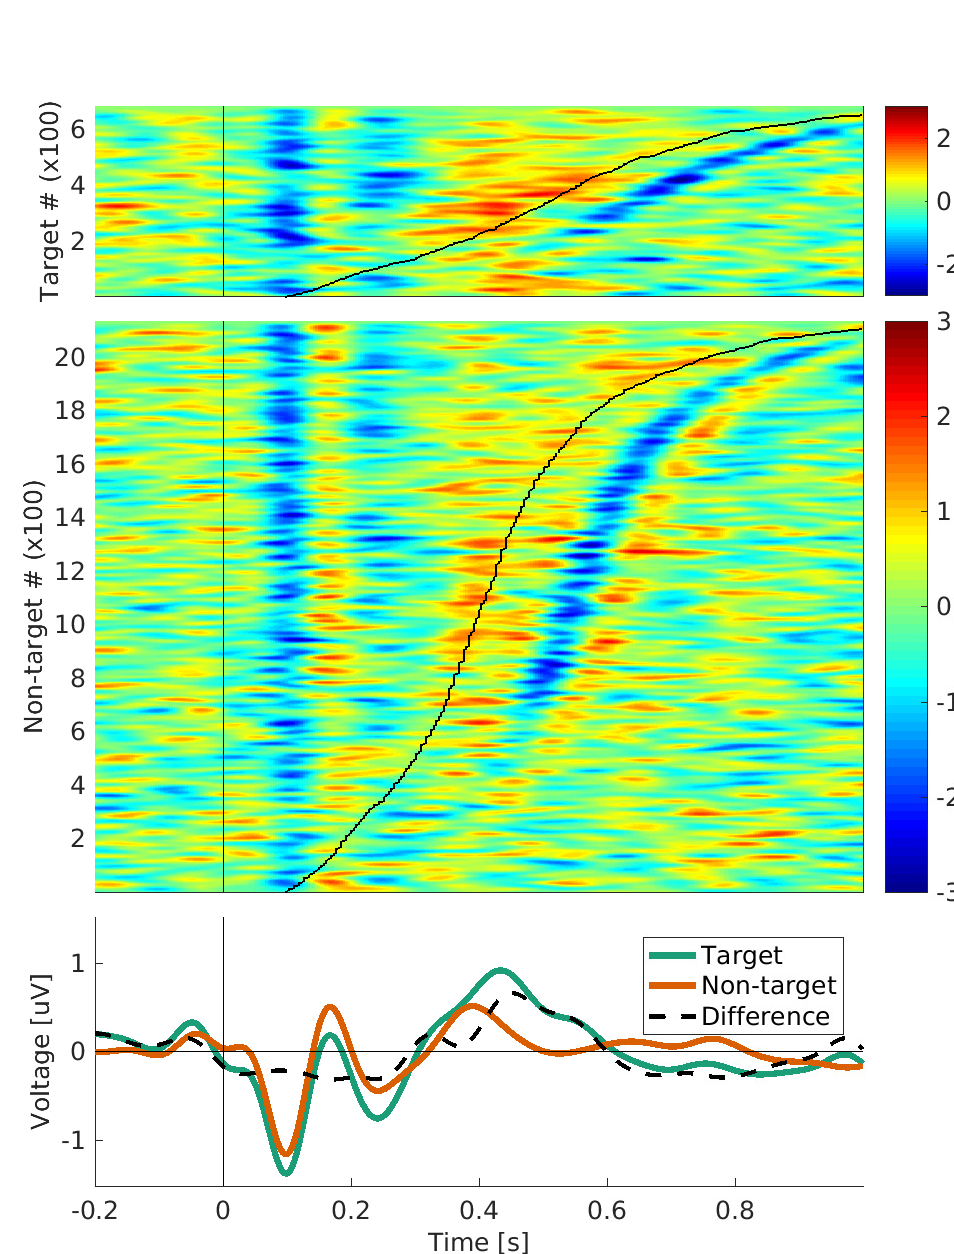
\includegraphics[trim={0cm 0cm 1.5cm 0cm},clip,width=0.45\columnwidth]{../images/offline/Epochs_GA_chCz_Saggregate_objrec_subjects_popuponline_s1.pdf}%
    %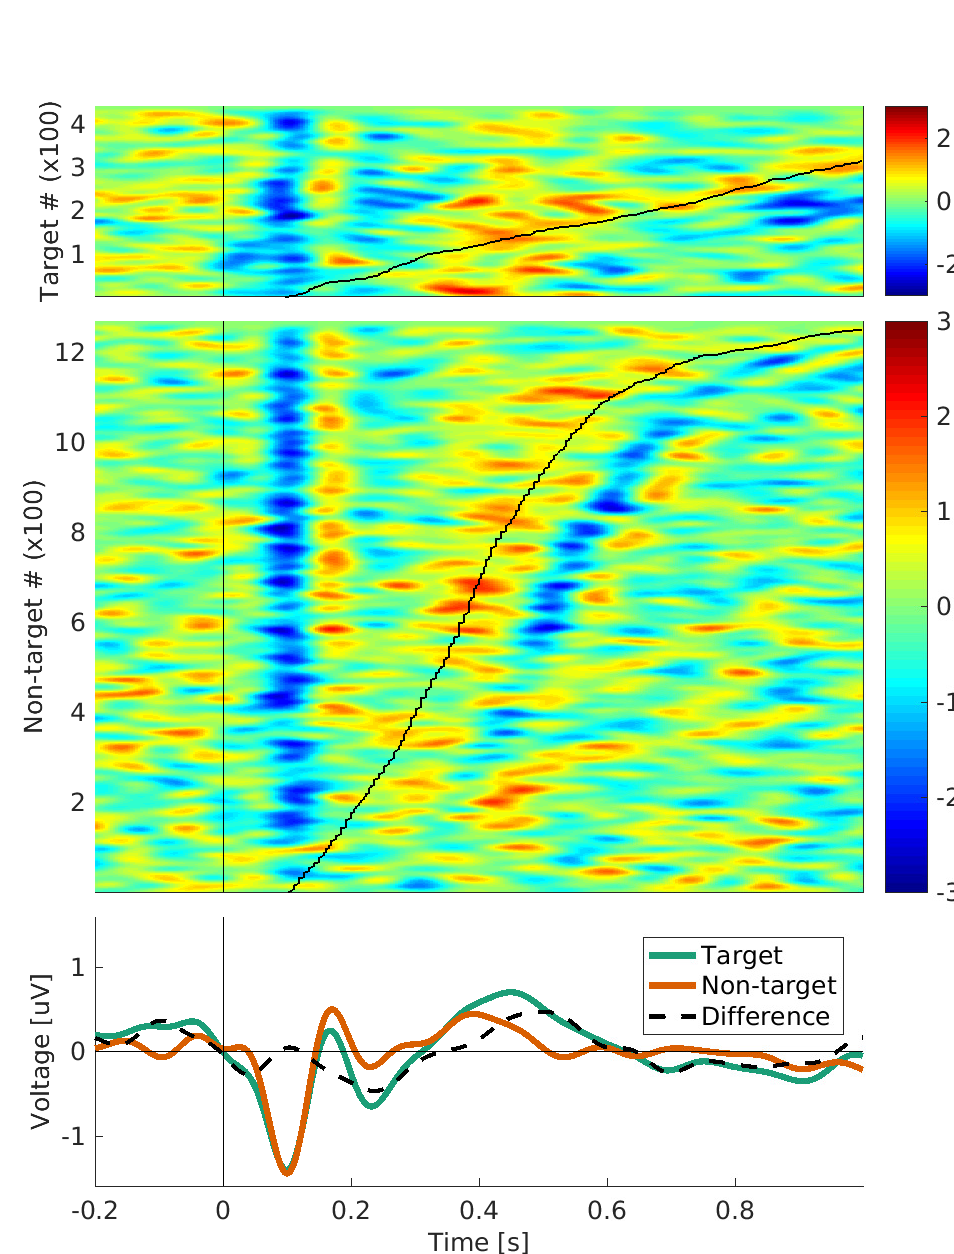
\includegraphics[trim={0cm 0cm 1.5cm 0cm},clip,width=0.45\columnwidth]{../images/online/Epochs_GA_chCz_Saggregate_objrec_subjects_popuponline_s1.pdf}%
    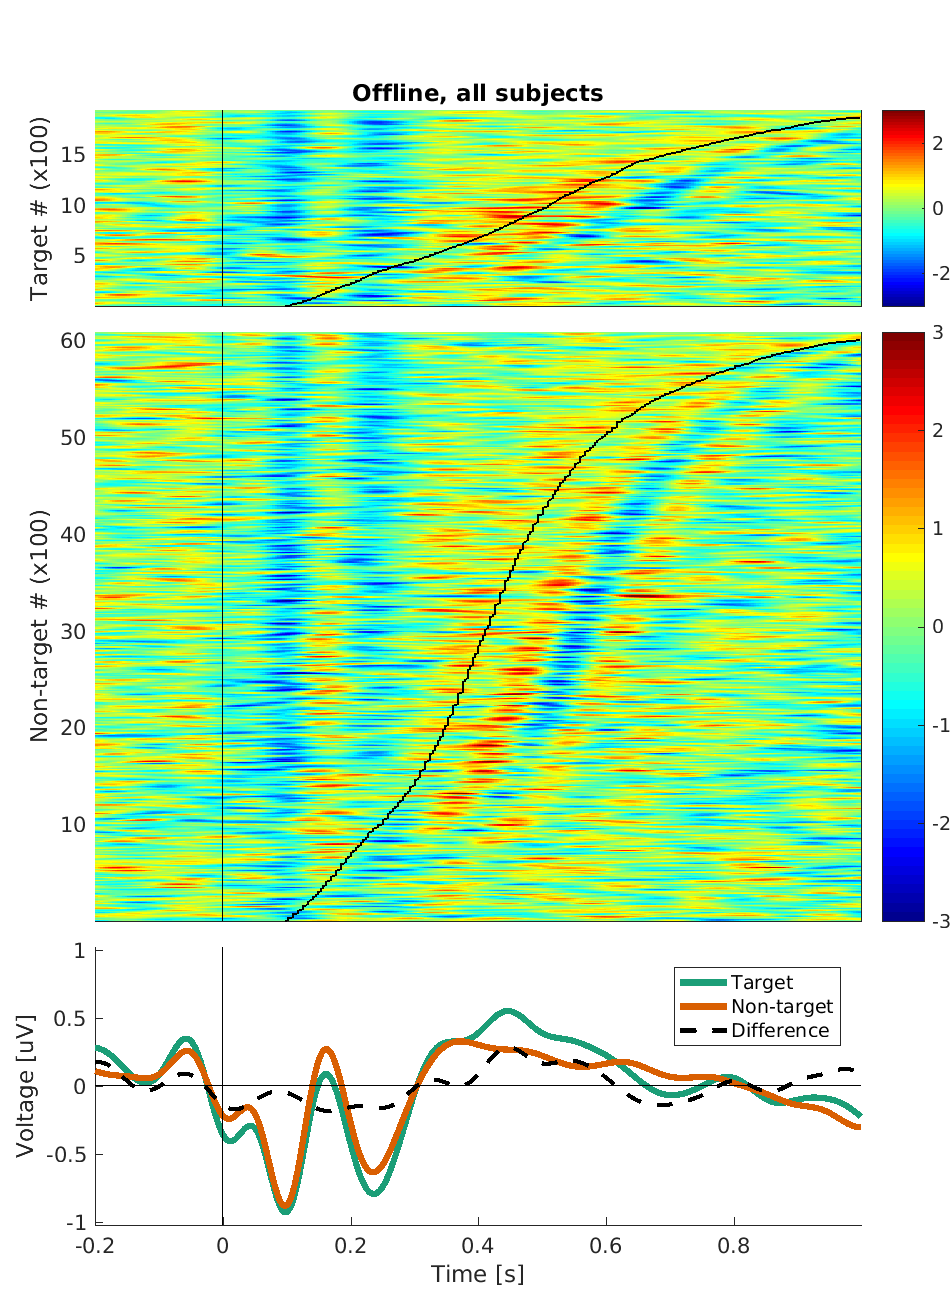
\includegraphics[trim={0cm 0cm 1.5cm 0cm},clip,height=0.65\columnwidth]{../images/Epochs_Offline_chCz_allsubjects.pdf}%
    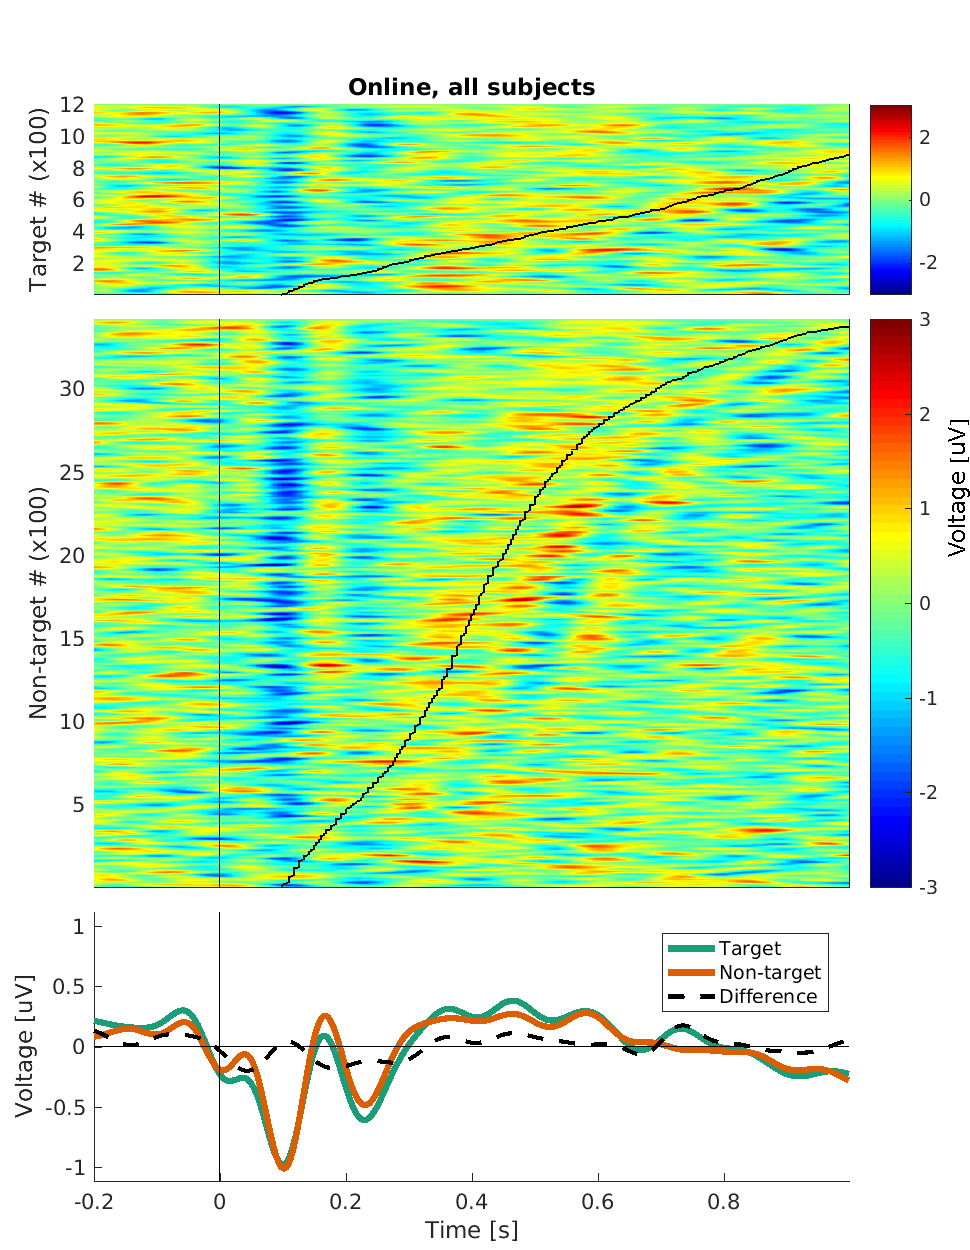
\includegraphics[trim={0cm 0cm 0cm 0cm},clip,height=0.65\columnwidth]{../images/Epochs_Online_chCz_allsubjects.pdf}%
    \caption{The signal of Cz channel for extracted EFRP epochs aggregated
        for all subjects.
        Left: offline phase. Right: online phase.
        Top panel: target EFRP epochs. Middle panel: non-target EFRP epochs.
        Bottom line plot: average signal across target and non-target EFRP epochs.
        The epochs are ordered according to the dwell time
        shown with the black S-shaped curve.
    }
%\label{fig:epochsCz}
%\end{figure}%

%\begin{figure}[h]
%\center
    \vspace{0.5cm}
    %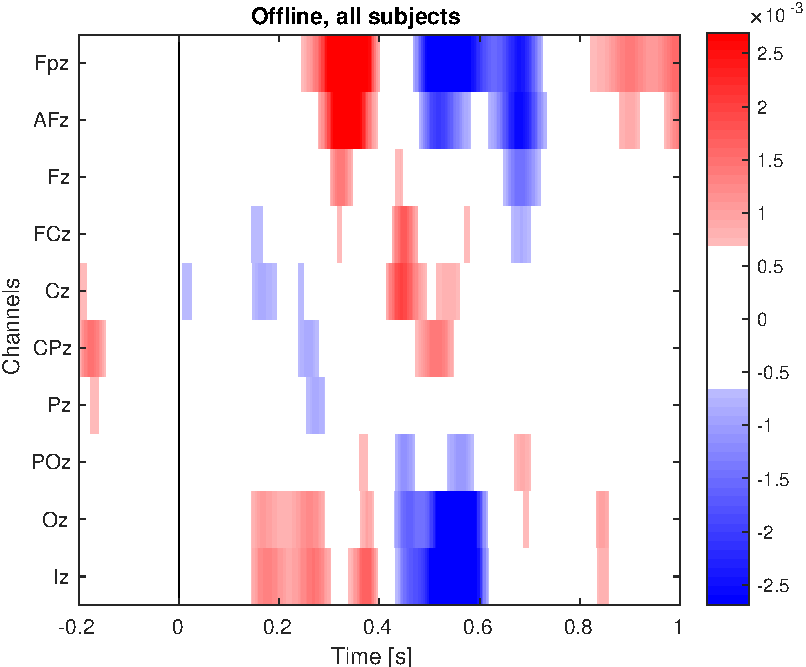
\includegraphics[trim={0cm 0cm 0cm 0cm},clip,width=0.45\columnwidth]{../images/Signr2_Offline_chCz_allsubjects.pdf}
    %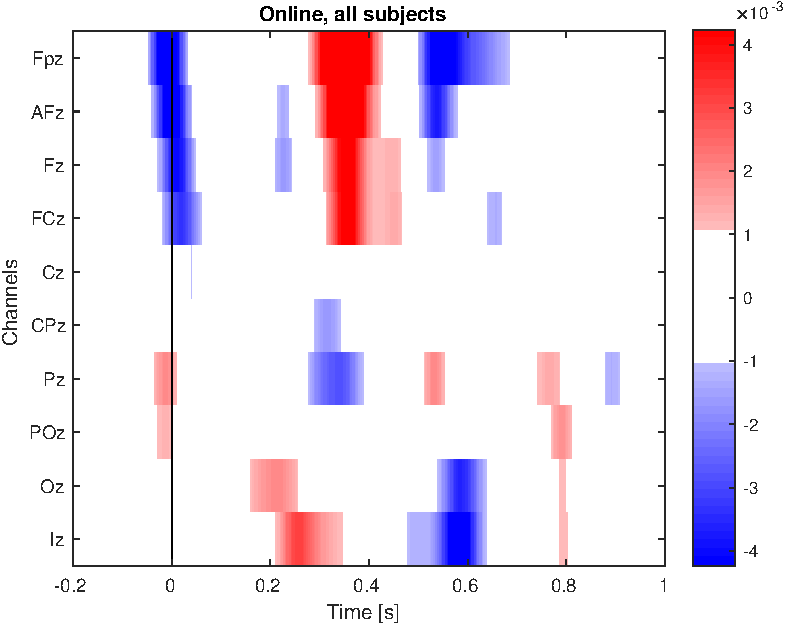
\includegraphics[trim={0cm 0cm 0cm 0cm},clip,width=0.45\columnwidth]{../images/Signr2_Online_chCz_allsubjects.pdf}
    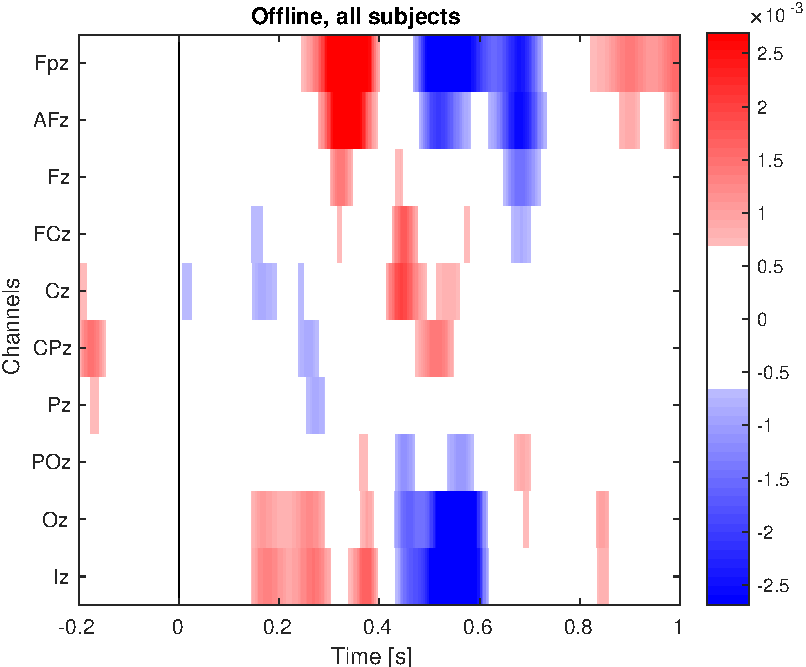
\includegraphics[trim={0cm 0cm 0cm 0cm},clip,height=0.4\columnwidth]{../images/Signr2_Offline_chCz_allsubjects.pdf}
    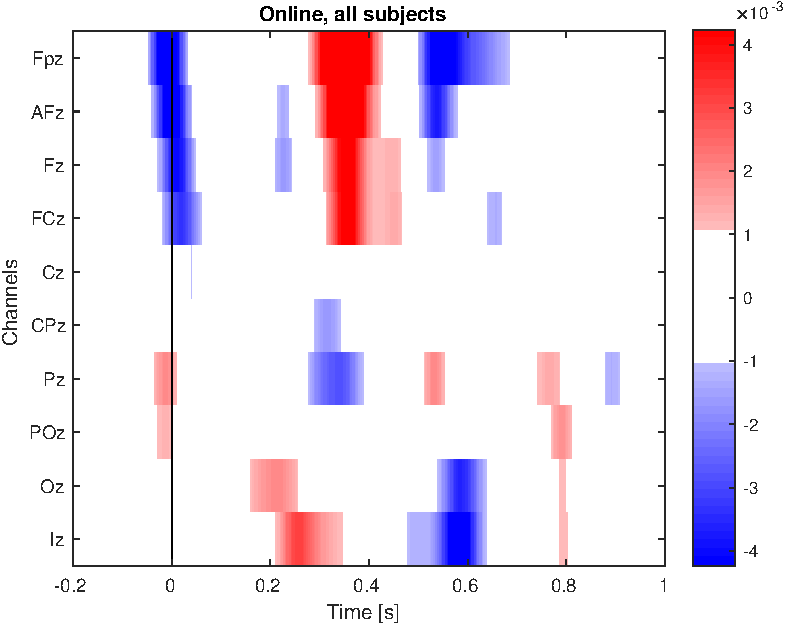
\includegraphics[trim={0cm 0cm 0cm 0cm},clip,height=0.4\columnwidth]{../images/Signr2_Online_chCz_allsubjects.pdf}
    \caption{The discriminant power for the aggregated epochs of
        all subjects.
    Signed $R^2$ is demonstrated for midline channels around the eye fixation onset
    (left: offline, right: online).}
\label{fig:signRtime}
\end{figure}

\begin{figure}[h]
\center
    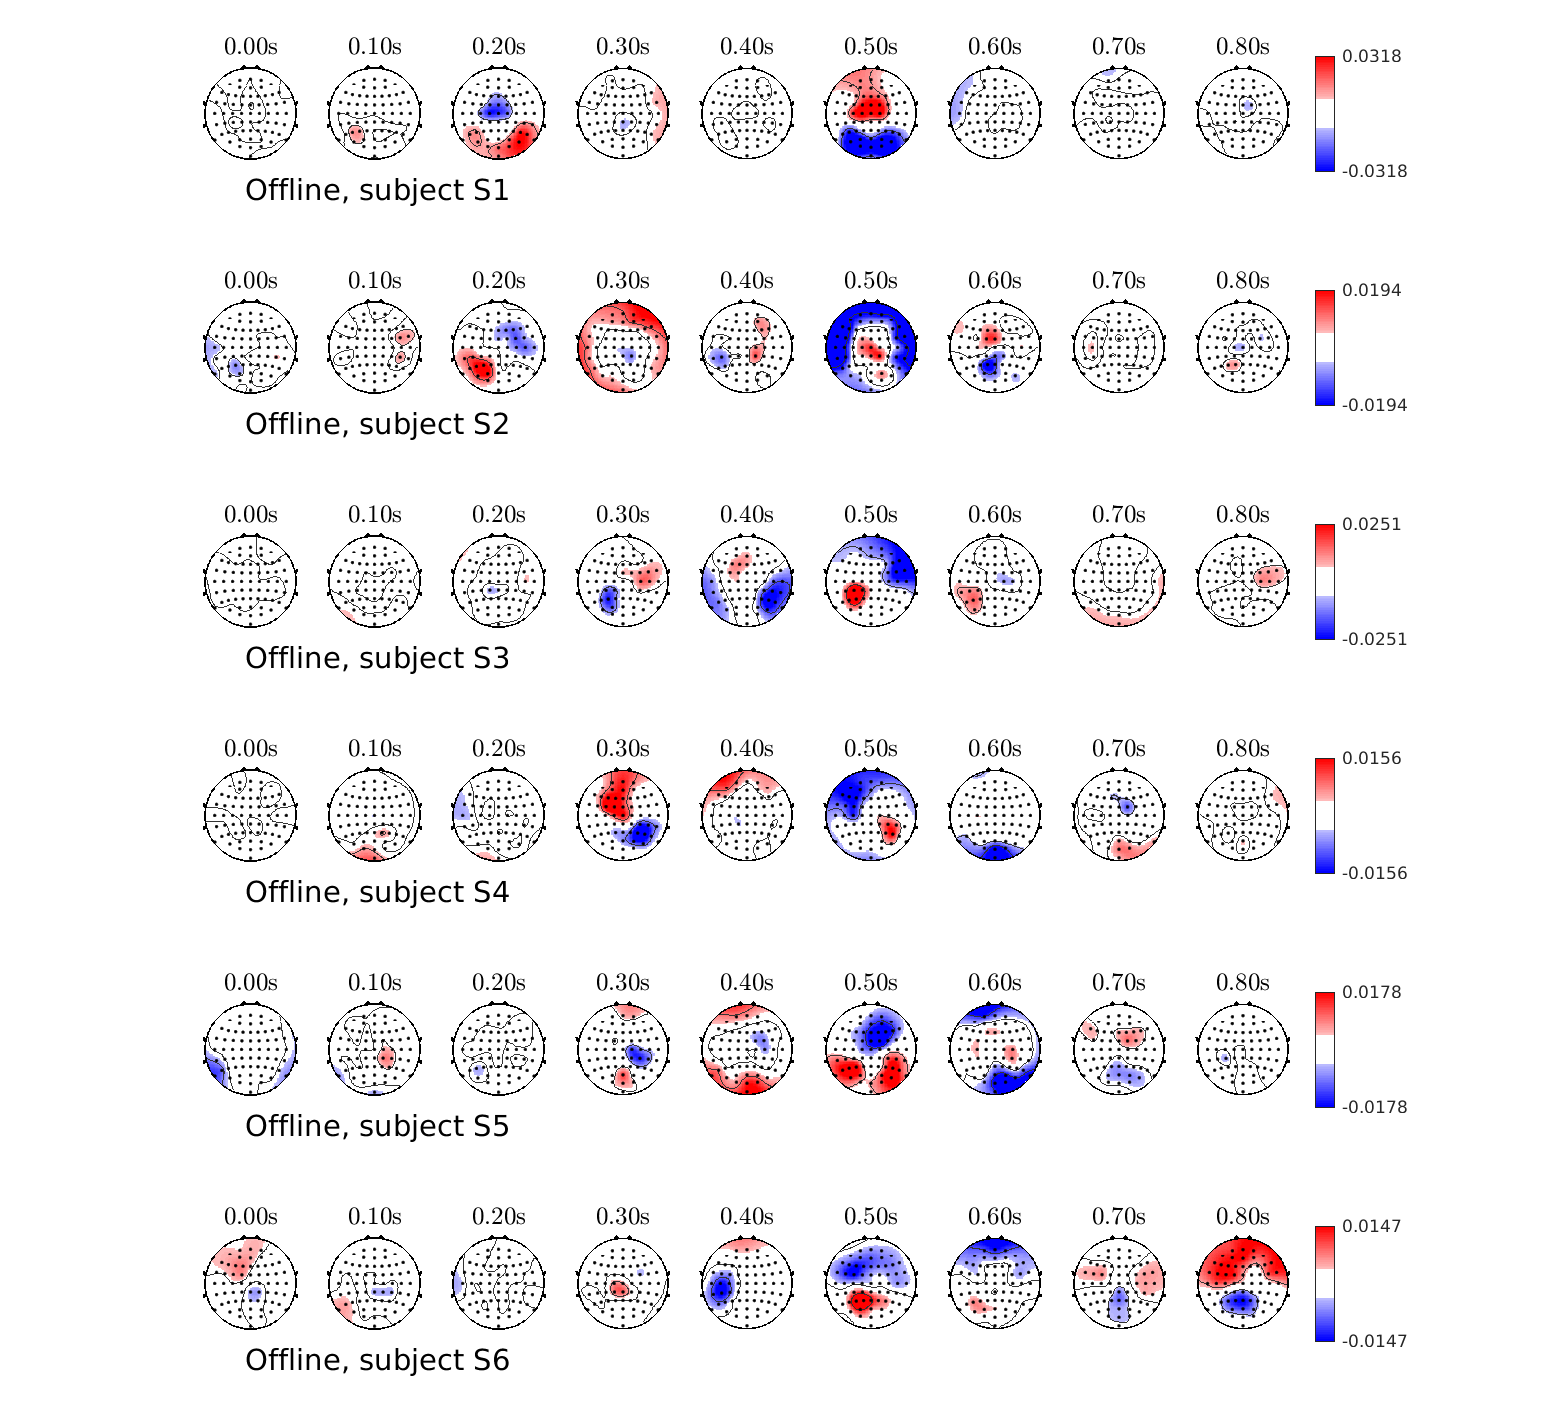
\includegraphics[trim={1cm 0.01cm 1cm 0cm},clip,width=1.0\columnwidth]{../images/TopoSignr2_Offline_individual1.png}
    \caption{The discriminant power (signed $R^2$) for subjects S1-S6 for the offline phase data.}
\label{fig:signRoff1}
\end{figure}

\begin{figure}[h]
\center
    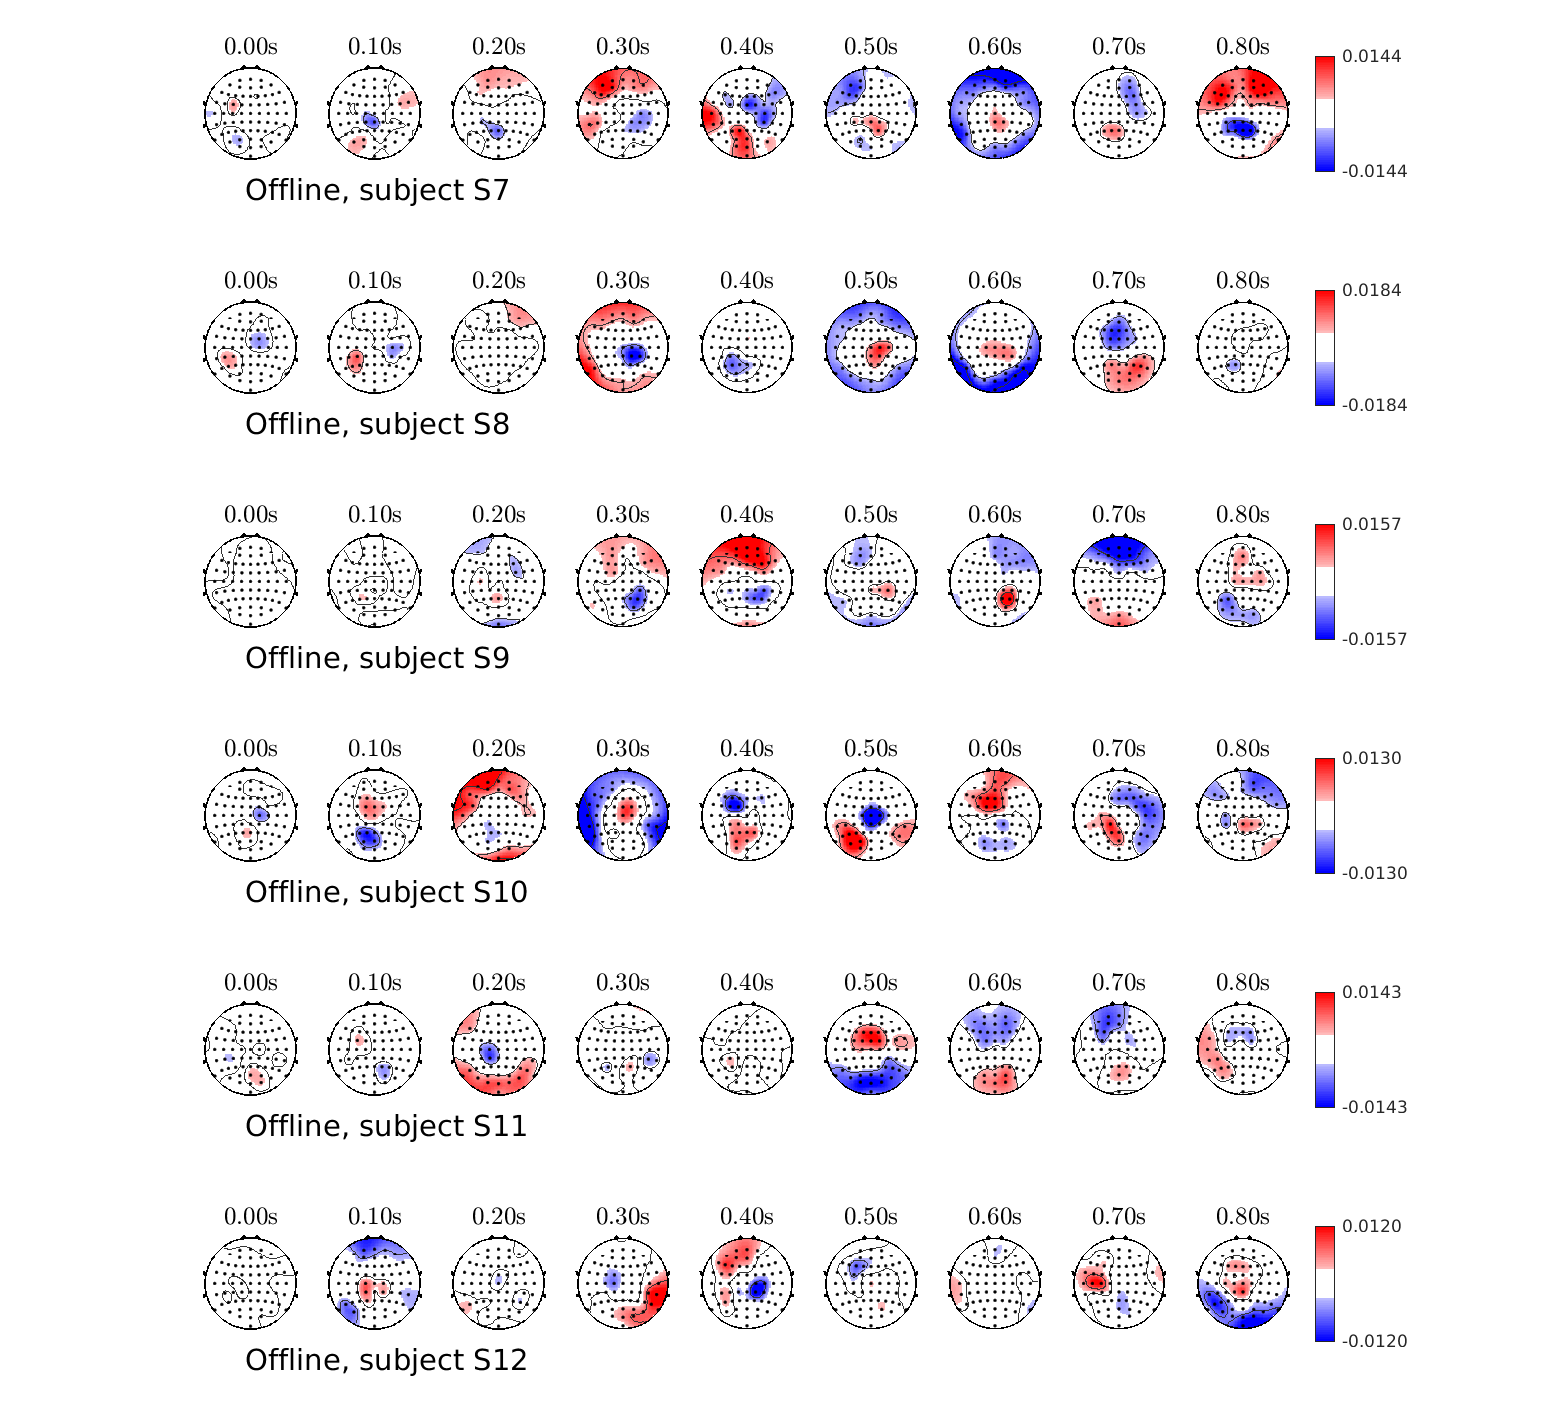
\includegraphics[trim={1cm 0.01cm 1cm 0cm},clip,width=1.0\columnwidth]{../images/TopoSignr2_Offline_individual2.png}
    \caption{The discriminant power (signed $R^2$) for subjects S7-S12 for the offline phase data.}
\label{fig:signRoff2}
\end{figure}

\begin{figure}[h]
\center
    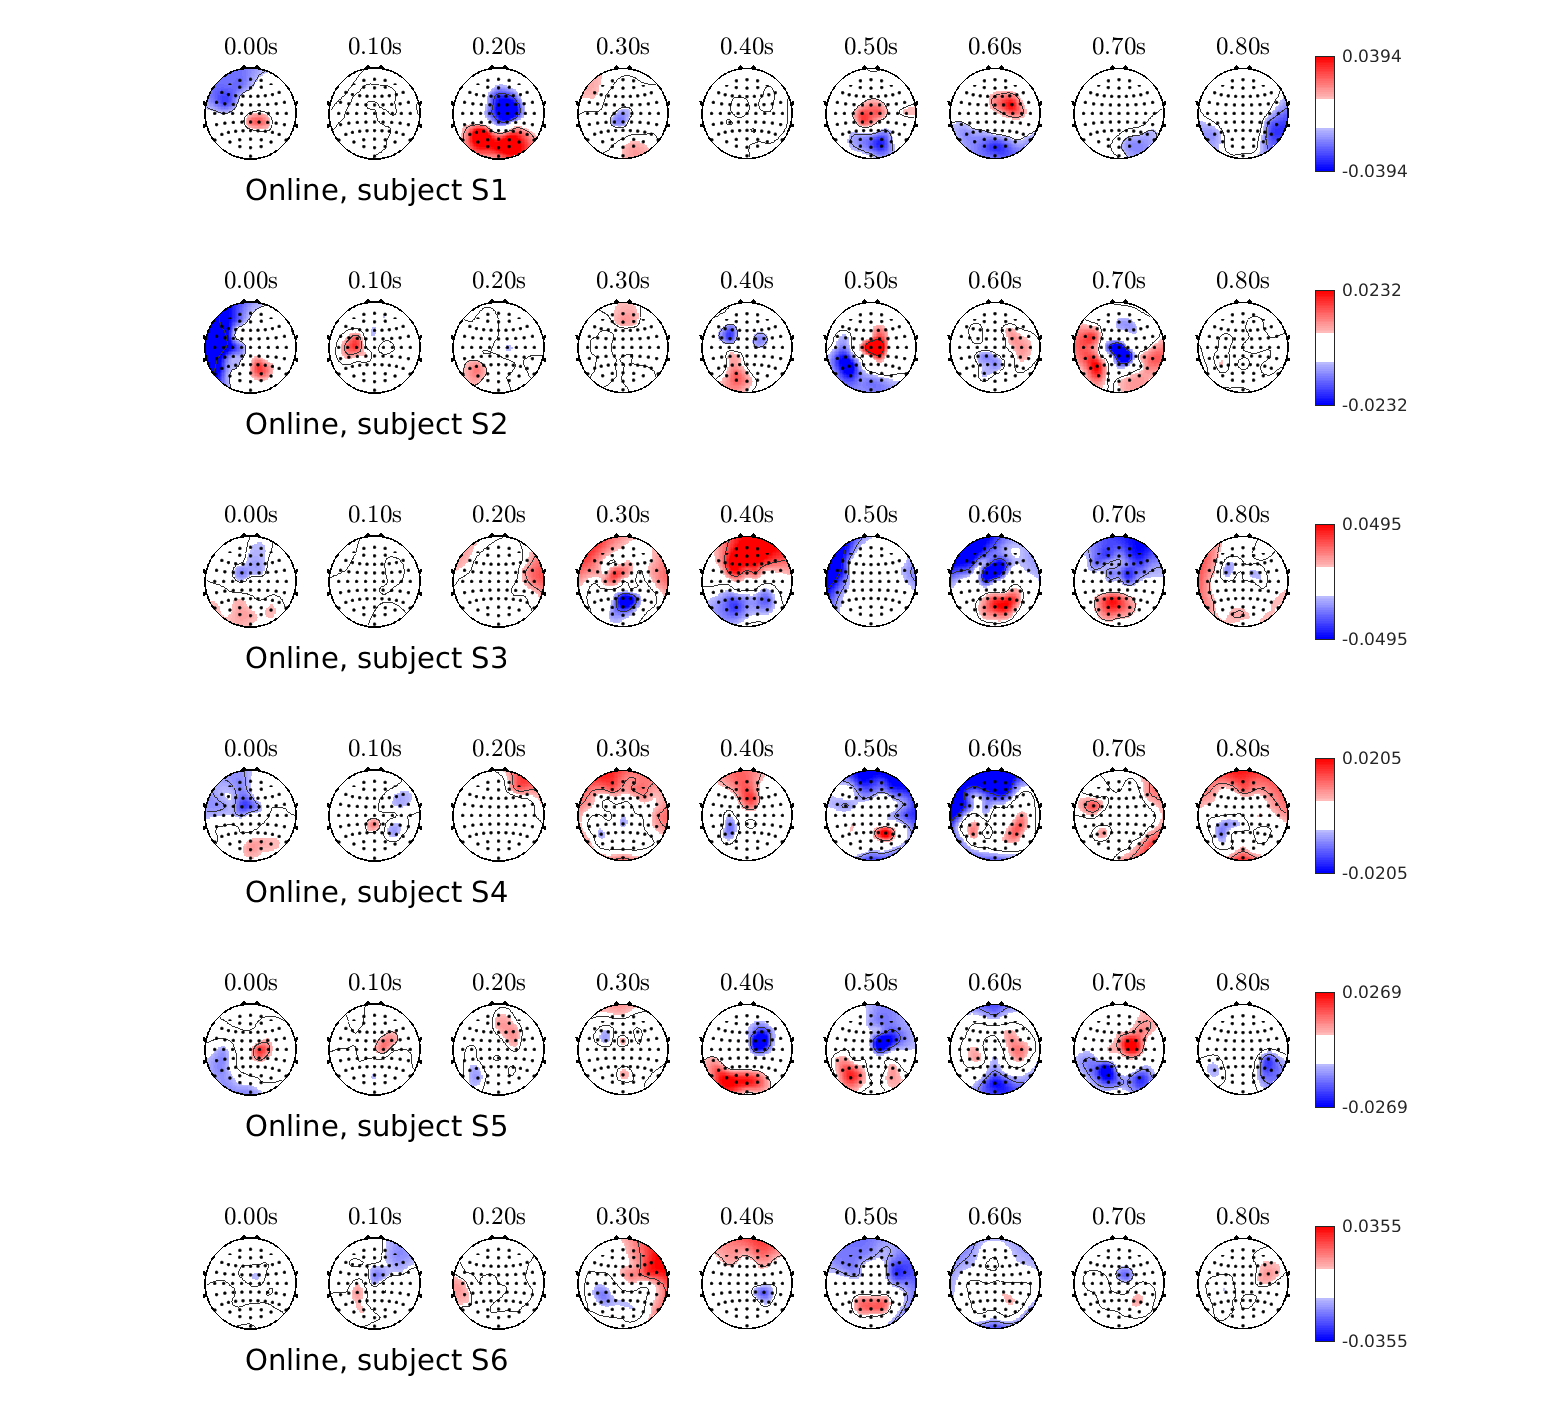
\includegraphics[trim={1cm 0.01cm 1cm 0cm},clip,width=1.0\columnwidth]{../images/TopoSignr2_Online_individual1.png}
    \caption{The discriminant power (signed $R^2$) for subjects S1-S6 for the online phase data.}
\label{fig:signRon1}
\end{figure}

\begin{figure}[h]
\center
    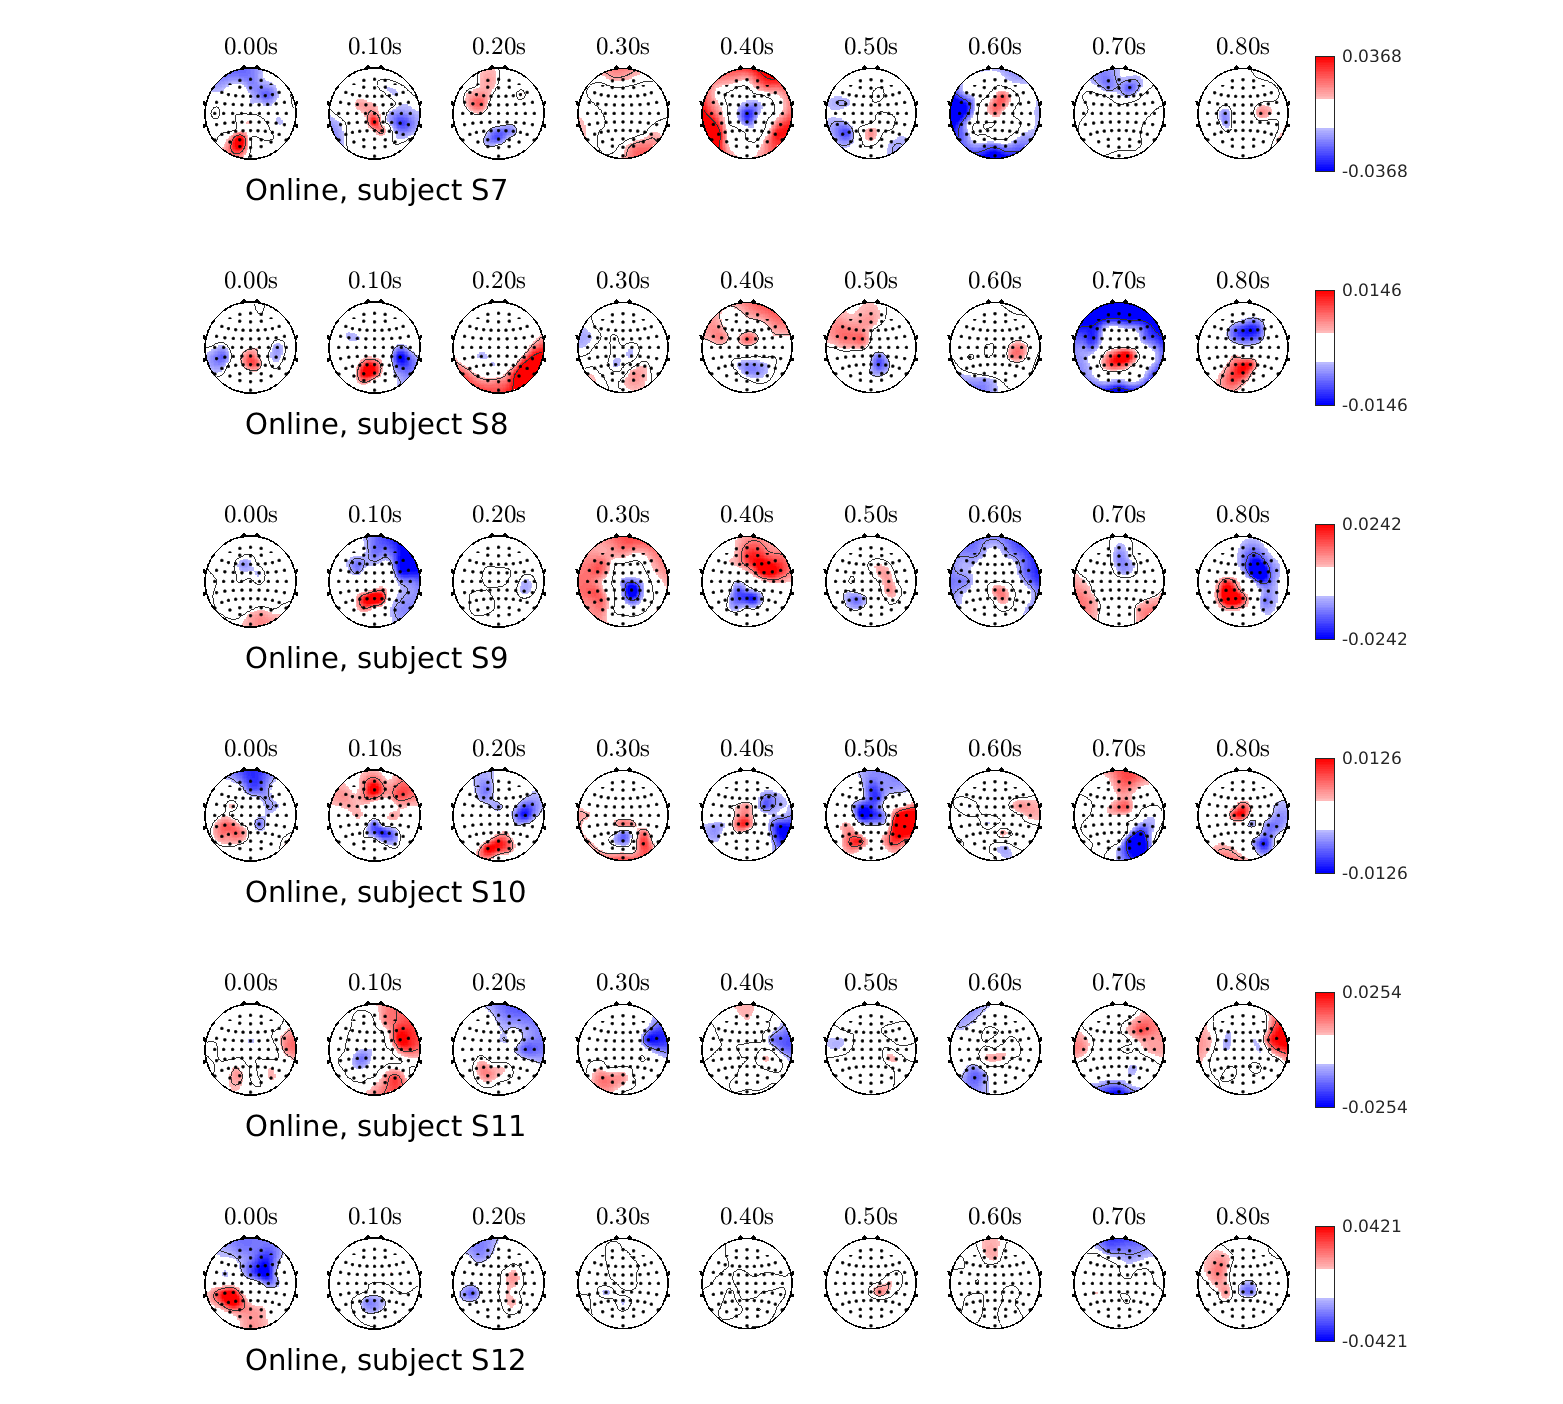
\includegraphics[trim={1cm 0.01cm 1cm 0cm},clip,width=1.0\columnwidth]{../images/TopoSignr2_Online_individual2.png}
    \caption{The discriminant power (signed $R^2$) for subjects S7-S12 for the online phase data.}
\label{fig:signRon2}
\end{figure}

\end{document}

